% Chapter X

\chapter{Arquitectura del CWC} % Chapter title

\label{ch:arquitectura_cwc} % For referencing the chapter elsewhere, use \autoref{ch:name} 

El enfoque del CWC consiste en conformar una comunidad alrededor de un sitio web, como cualquier otra comunidad virtual que se crea en Internet. 

Por ejemplo, una comunidad que se conforma alrededor de la música de un género, en esta comunidad los usuarios aportan nuevas canciones para ser compartidas por el resto de los usuarios. Es dinámica, los miembros van y vienen.

Es fácil concluir que, una comunidad virtual se reúne alrededor de algún interés en común  y ayudan para que esta comunidad se mantenga con el tiempo. La idea es principal del CWC  es que los usuarios de un sitio web, se conviertan en pequeñas cachés de éste y de esta manera poder hacer que el sitio web pueda servir a más usuarios. 

Como se puede observar en la figura \ref{ComunidadWebCache}, los usuarios de un sitio web específico forman parte de la comunidad de éste, donde aportan recursos que se utilizan para mantener una caché de ciertos archivos, los cuales son servidos desde las cachés en lugar de ser servidos desde el servidor principal.

\begin{figure}[h]
  \centering
    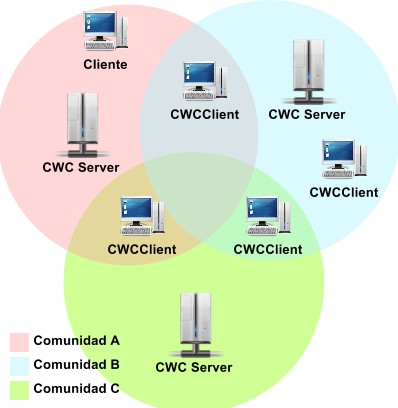
\includegraphics[scale=0.5]{gfx/ComunidadWebCache}
  \caption{Comunidad Web Caché}
  \label{ComunidadWebCache}
\end{figure}

En esta sección se describirá la arquitectura que seguirá cada una de las partes que conforman el CWC.
%----------------------------------------------------------------------------------------

\section{CWC Server}

En la figura \ref{ComunicacionCWCServer}, se puede observar el esquema de una comunicación utilizando CWC, esta comunicación debe ser transparente, de manera que un usuario que no utilice CWC será atendido directamente por el servidor web, en el caso de que un cliente si la utilice entonces esta será atendida por la comunidad  y el servidor. 


\begin{figure}[h]
  \centering
    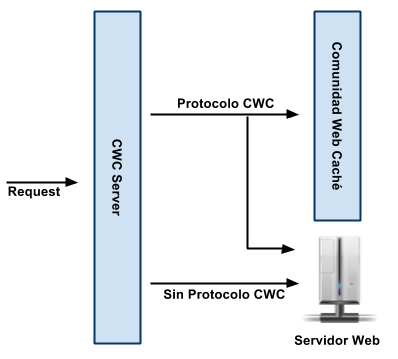
\includegraphics[scale=0.75]{gfx/ComunicacionCWCServer}
  \caption{Comunicación del CWC Server}
  \label{ComunicacionCWCServer}
\end{figure}


Por otro lado, como se puede observar en la figura \ref{ArquitecturaCWCServer}, se presenta una arquitectura multicapa, en los siguientes apartados se explicará cada una de las capas y la interacción entre ellas.

\begin{figure}[h]
  \centering
    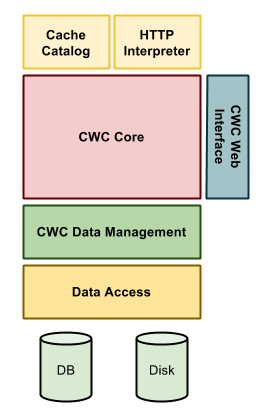
\includegraphics[scale=0.75]{gfx/ArquitecturaCWCServer}
  \caption{Arquitectura CWC Server}
  \label{ArquitecturaCWCServer}
\end{figure}

%------------------------------------------------

\subsection{Data Access}

La capa de acceso a datos implementa toda la lógica para realizar el acceso a datos en este caso se deberá implementar para el acceso para:

\begin{enumerate}
\item Base de datos: En el caso de la base de datos, este será el repositorio donde se almacenarán las estadísticas y la información de los objetos y los miembros de la CWC.
\item Disco: En este caso se trata de archivos planos de texto, de acceso secuencial que se utilizaran para almacenar logs de acceso, logs del CWC Server en general. Los logs de acceso serán analizados una vez a la semana y se almacenarán en la base de datos. Este proceso no se realiza de forma continua pues es necesario reducir el tráfico al disco y utilizar la mínima cantidad de recursos.
\end{enumerate}

%------------------------------------------------

\subsection{CWC Data Management}

El CWC Data Management, actuará como una caché para la base de datos, contendrá la información que se está utilizando  de la base de datos actualmente, más la información que se está generando por el uso del sistema. Las estructuras permanecerán en memoria y actuarán como si fuesen la capa de acceso a datos, pero en realidad todo se estará trabajando desde la  memoria. 

Periódicamente se realizará una descarga de toda esta información hacia la base de datos. La justificación para hacerlo de esta manera es para disminuir la cantidad de accesos a la base de datos y tener la información requerida en memoria para ser accedida de manera rápida y reducir el gasto adicional debido al uso de CWC. En lo referente a logs, éstos ingresarán directamente a disco, pues esta información es de solo lectura y no será analizada en tiempo real para tomar decisiones. 

El tiempo entre cada descarga será definido por el administrador del sitio web, hay que tomar en cuenta que debido a que esta información se va a mantener en memoria volátil, ésta se puede perder, pero este es un riesgo que se asumirá en favor de brindar un mejor servicio. 

Debido a que el periodo de tiempo entre cada descarga es configurable, si se desea reducir el riesgo de perder información, este tiempo deberá tender a ser corto, de lo contrario, puede ser tan largo como se desee. 


%----------------------------------------------------------------------------------------

\subsection{CWC Core}

En la capa CWC Core es donde se implementa toda la funcionalidad de la Comunidad Web Caché, en esta capa se implementará:

\begin{itemize}
\item Administración de Objetos Cacheables.
\item Administración de miembros de la CWC.
\item Administración de estadísticas.
\item Se contará con un módulo para toma de decisiones en base a las estadísticas recolectadas.
\item Comunicación con el servidor web.
\item Comunicación con los miembros de las caches.
\end{itemize}

La capa CWC Core implementará toda la funcionalidad fundamental de la Comunidad Web Caché, ésta tendrá interacción con:
\begin{itemize}
\item La capa CWC Data Management para escribir y leer datos.
\item La capa CWC Web Interface para comunicarse con el servicio web.
\item La capa CWC HTTP Interpreter para recibir las peticiones, analizarlas y determinar si éstas son válidas y utilizan el Protocolo CWC. Además enviará mensajes utilizando el este mismo protocolo.
\item La capa CWC Cache Catalog para comunicarse con las caches, para recibir y enviar mensajes con estas, tendrá una conexión permanente con éstas para realizar la comunicación.
\end{itemize}

\subsection{CWC Caches Catalog}
Esta capa es la que se encarga de tener una conexión permanente con las caches y también de intercambiar cualquier mensaje con éstas, es el módulo que se comunica a través del protocolo CWC, está constantemente intercambiando mensajes con las cachés para recolectar estadísticas, para indicar cambios de estados en los objetos, entre otros. 

\subsection{CWC Protocol Interpreter}
En esta capa se realiza el análisis de cualquier petición utilizando el protocolo HTTP,  se identifica si la petición utiliza correctamente el protocolo CWC, si es así se pasa el mensaje a la capa CWC Core para que sea atendida. Cuando su atención termine recibirá la respuesta y la enviará al cliente que realizó la petición, en el caso de que la petición no utilice el protocolo CWC será enviada al CWC Web Interface que actuará como un simple puente hacia el servidor web.

\subsection{CWC Web Interface}
Como se ha mencionado anteriormente, el CWC Server se implementará como un módulo de un servidor web existente. 

Este módulo será una capa que actuará como un interfaz para intercambiar datos con las estructuras internas del servicio web y para reenviar las solicitudes que deban ser atendidas por éste.

\section{CWC Client}
En la figura \ref{ComunicacionCWCClient} se muestra el esquema general del mecanismo de comunicación del CWC Client. Este actuará como un "proxy web cache" para las peticiones que envía el cliente. 

Por ejemplo, si se envía una petición a http://www.cwc.com esta petición será interceptada por el CWC Client y resuelta mediante el protcolo CWC, al final el CWC Client se encarga de obtener el archivo desde las diferentes cachés y ensamblarlo, además también se ocupa de servirlo al navegador web. El uso de una Comunidad Web Caché es totalmente trasparente para el usuario y el navegador web. Una versión más detallada de lo que sucede es la siguiente:

\begin{enumerate}
\item El CWC Client, intercepta la petición.
\item Se verifica que el Servidor Web utilice el protocolo CWC.
\item En el caso de que no se utilice, se realizará la petición directamente al servidor.
\item En el caso de que se utilice, se solicitará la lista de cachés con el objeto al servidor.
\item Se inicia la descarga distribuida.
\item Se vuelve a ensamblar el archivo una vez que se tengan todas las partes.
\item Se envía el resultado al navegador web.
\end{enumerate}

\begin{figure}
  \centering
    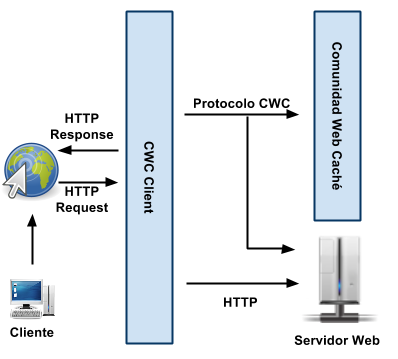
\includegraphics[scale=0.75]{gfx/ComunicacionCWCClient}
  \caption{Comunicación del CWC Client}
  \label{ComunicacionCWCClient}
\end{figure}

La arquitectura del CWC Client es muy similar al de CWC Server. En la figura \ref{ArquitecturaCWCClient} se muestra una descripción gráfica, donde las principales diferencias radican en:

\begin{enumerate}
\item No cuenta con una base de datos.
\item No cuenta con un servidor web. 
\item Funcionará como una extensión para el navegador web. 
\end{enumerate}

\begin{figure}
  \centering
    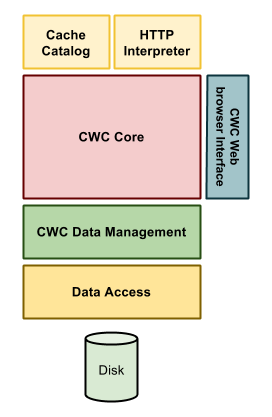
\includegraphics[scale=0.75]{gfx/ArquitecturaCWCClient}
  \caption{Arquitectura CWC Client}
  \label{ArquitecturaCWCClient}
\end{figure}

\subsection{Data Access}
En esta capa se implementará toda la lógica para el acceso a datos, en este caso solo se realizarán accesos a disco, por lo mencionado anteriormente, pues no cuenta con una base de datos del lado del cliente y además porque la principal funcionalidad de ésta es realizar la transmisión de archivos a disco. 

\subsection{CWC Data Management}
Esta capa también como en el CWC Server, funciona como una cache de los datos, esto para reducir los accesos a disco que son sumamente costos.
En caso que un archivo sea leído desde multiples localizaciones, éste acceso se agilizará a través un la memoria de acceso aleatoria (RAM).

\subsection{CWC Client Core}
La capa CWC Client Core, implementará toda la funcionalidad básica de la Comunidad Web Caché, como lo es:

\begin{enumerate}
\item Interacción con el navegador web o agente de usuario.
\item Administración de la cache.
\item Verificación de Consistencia.
\item Administración de la membresía a la comunidad.
\item Servir un archivo.
\end{enumerate}

\subsection{CWC Cache Catalog}
Esta capa implementa el protocolo CWC en forma pura, cuando se trata de una caché, ésta capa se encarga de realizar toda la comunicación entre la cache y el servidor, mantiene una conexión con el servidor e intercambia mensajes. 

\subsection{CWC HTTP Interpreter}
Esta capa implementa de manera muy básica el protocolo HTTP, sirve como cliente para hacer los HTTP Distributed Get y para servir partes de archivos. Además sus funciones son:
\begin{enumerate}
\item Realizar las peticiones HTTP.
\item Servir Archivos.
\end{enumerate}

\subsection{CWC Web Browser Interface}
Esta se encarga de integrarse con la arquitectura del navegador web o el agente de usuario, en este caso se integra para capturar todas las peticiones HTTP y enviarlas en formato CWC.